% HW Template for CS 6150, taken from https://www.cs.cmu.edu/~ckingsf/class/02-714/hw-template.tex
%
% You don't need to use LaTeX or this template, but you must turn your homework in as
% a typeset PDF somehow.
%
% How to use:
%    1. Update your information in section "A" below
%    2. Write your answers in section "B" below. Precede answers for all 
%       parts of a question with the command "\question{n}{desc}" where n is
%       the question number and "desc" is a short, one-line description of 
%       the problem. There is no need to restate the problem.
%    3. If a question has multiple parts, precede the answer to part x with the
%       command "\part{x}".
%    4. If a problem asks you to design an algorithm, use the commands
%       \algorithm, \correctness, \runtime to precede your discussion of the 
%       description of the algorithm, its correctness, and its running time, respectively.
%    5. You can include graphics by using the command \includegraphics{FILENAME}
%
\documentclass[11pt]{article}
\usepackage{amsmath,amssymb,amsthm}
\usepackage{graphicx}
\usepackage[margin=1in]{geometry}
\usepackage{fancyhdr}
\usepackage{algorithm}
\usepackage{algpseudocode}
\usepackage{pifont}
\setlength{\parindent}{0pt}
\setlength{\parskip}{5pt plus 1pt}
\setlength{\headheight}{13.6pt}
\newcommand\question[2]{\vspace{.25in}\hrule\textbf{#1: #2}\vspace{.5em}\hrule\vspace{.10in}}
\renewcommand\part[1]{\vspace{.10in}\textbf{(#1)}}
\newcommand\algorith{\vspace{.10in}\textbf{Algorithm: }}
\newcommand\correctness{\vspace{.10in}\textbf{Correctness: }}
\newcommand\runtime{\vspace{.10in}\textbf{Running time: }}
\pagestyle{fancyplain}
\lhead{\textbf{\NAME\ (\UID)}}
\chead{\textbf{HW\HWNUM}}
\rhead{CS 6350, \today}
\begin{document}\raggedright
%Section A==============Change the values below to match your information==================
\newcommand\NAME{Jake Pitkin}  % your name
\newcommand\UID{u0891770}     % your utah UID
\newcommand\HWNUM{5}              % the homework number
%Section B==============Put your answers to the questions below here=======================

\question{1}{Margins}

\part{1} Consider the following input to the XOR function in two dimensions ($x_1, x_2$) and the input mapped into the space ($x_1, x_1x_2$).

 \begin{table}[H]
\centering
{\renewcommand{\arraystretch}{1.2}%
\begin{tabular}{| c | c | c | c |}
\hline
$x_1$ & $x_2$ & label & $x_1x_2$\\
\hline
-1 & -1 & -1 & 1\\ \hline
-1 & 1 & 1 & -1\\ \hline
1 & -1 & 1& -1 \\ \hline
1 & 1 & -1 & 1\\ \hline
\end{tabular}}
\caption{Inputs to the XOR function in two dimensions and mapping.}
\end{table}

\begin{figure}[H]
  \centerline{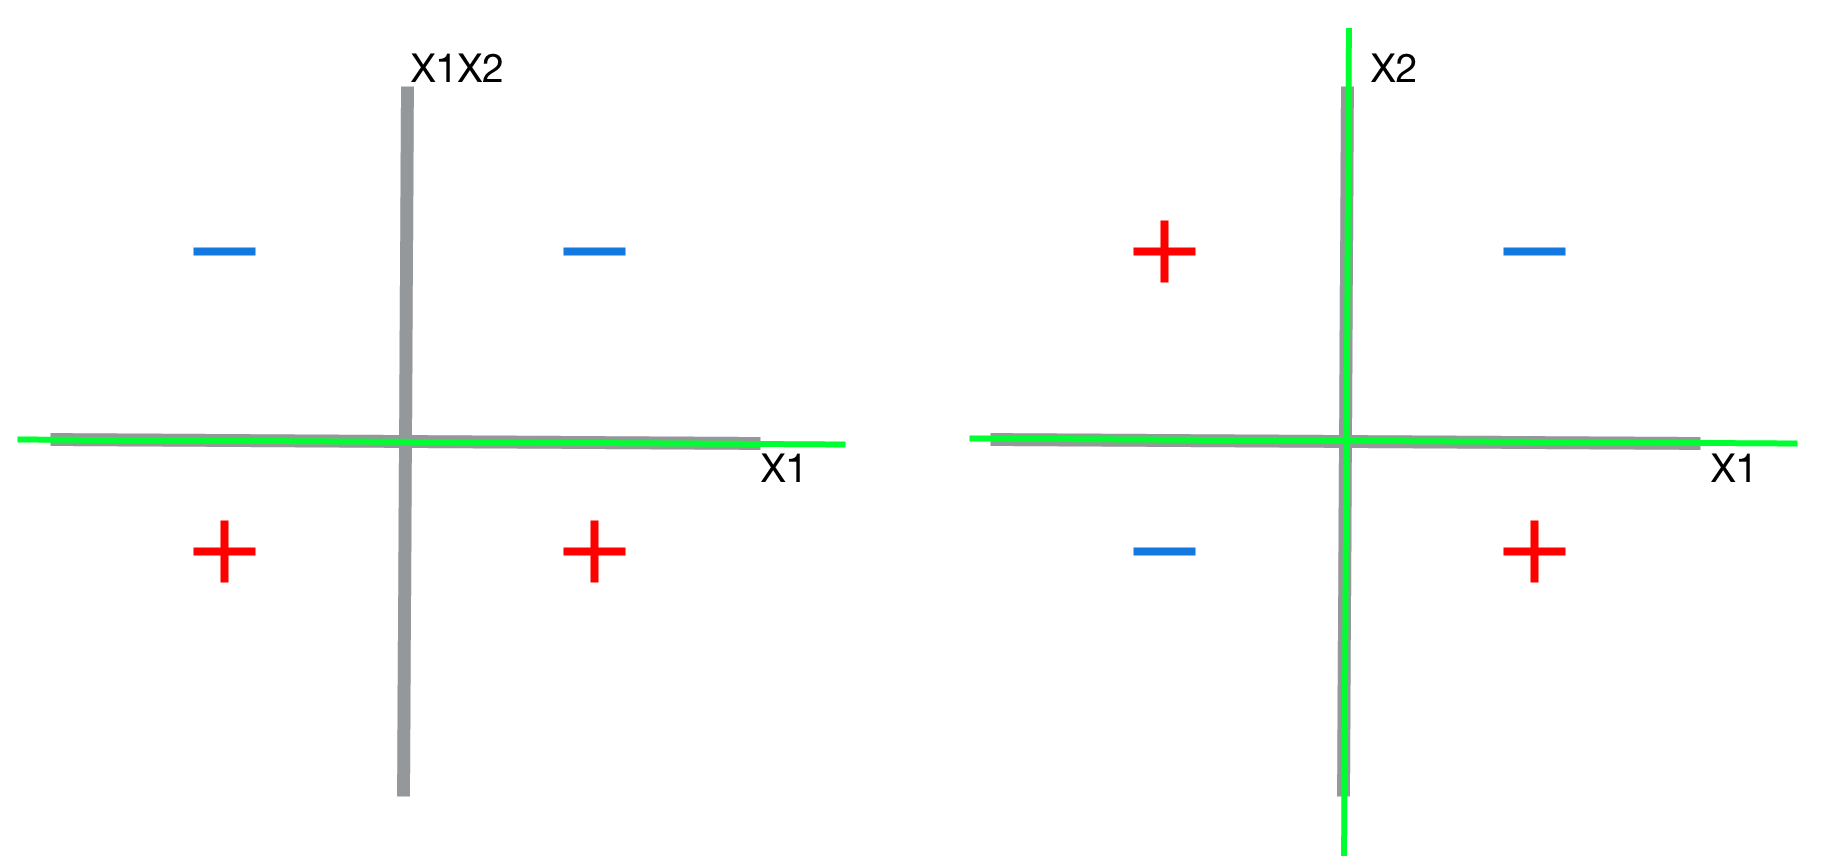
\includegraphics[width=0.8\linewidth]{1_1.png}}
  \caption{The separating line producing the maximal margin in both spaces.}
\end{figure}

The XOR function in $x_1, x_1x_2$ space has a maximum margin of 1. This is achieved with the separating line $x_1x_2 = 0$.

Translating the line $x_1x_2 = 0$ back to the original $x_1, x_2$ Euclidean space will be the lines $x_1 = 0$ and $x_2 = 0$. This is because $x_1x_2 = 0$ is true when at least one of $x_1$ or $x_2$ is 0. Which is satisfied by the lines running along the x1-axis and the x2-axis.

\framebox[1.2\width]{Maximum margin of 1.} 

\begin{figure}[H]
  \centerline{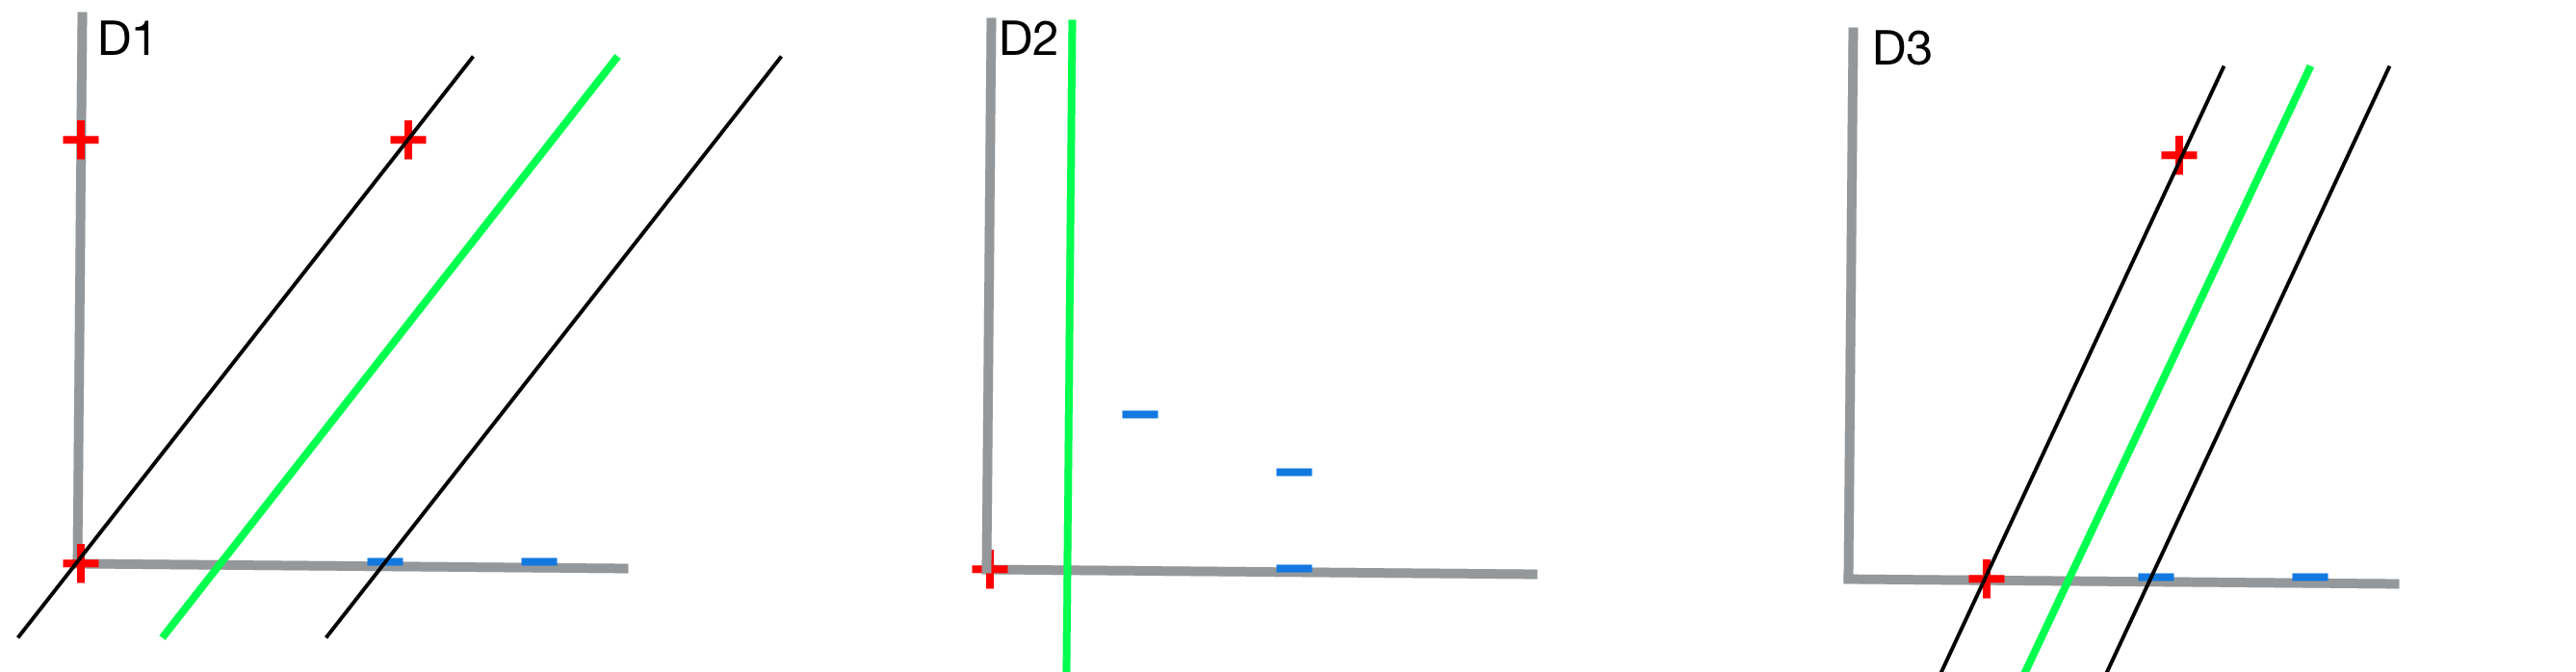
\includegraphics[width=0.8\linewidth]{1_2.png}}
  \caption{Geometry of the three training sets.}
\end{figure}

\part{2a} \textbf{$D_1$ - } Points $x_1$ and $x_3$ form the line $y - x = 0$ which has a slope of $1$. A line with slope $1$ that passes through point $x_5$ is given by $y - x + 1 = 0$. The parallel separating line between these two lines will give the maximum margin. It intersects the x-axis at ($0.5, 0$), has a slope of $1$ and is given by the formula $y - x + 0.5 = 0$. We can use the distance formula for a line and a point to determine the margin between this separating line and the nearest points.

\begin{equation}
\setlength\fboxsep{0.25cm}
\setlength\fboxrule{0.4pt}
\boxed{distance(ax + by + c = 0, (x_0, y_0)) = \frac{|ax_0 + by_0 + c|}{\sqrt{a^2 + b^2}}}
\end{equation} 

The separating line is defined by $a = -1$, $b = 1$, and $c = 0.5$.
$$distance(-x + y + 0.5 = 0, (0, 0)) = \frac{0.5}{\sqrt{2}}$$
$$distance(-x + y + 0.5 = 0, (1, 1)) = \frac{0.5}{\sqrt{2}}$$
$$distance(-x + y + 0.5 = 0, (1, 0)) = \frac{0.5}{\sqrt{2}}$$

\framebox[1.2\width]{$maximum \ \gamma = \frac{1}{2\sqrt{2}}$}

\textbf{$D_2$ - } The separating line that produces the maximum margin is evident from the geometry of the training points. As seen in figure 2, the line $x = 0.25$ separates the points with the maximum margin.

The separating line is defined by $a = 1$, $b = 0$, and $c = -0.25$.
$$distance(x - 0.5 = 0, (0, 0)) = 0.25$$
$$distance(x - 0.5 = 0, (\frac{1}{2}, \frac{\sqrt{3}}{2})) = 0.25$$

\framebox[1.2\width]{$maximum \ \gamma = 0.25$}

\textbf{$D_3$ - } Points $x_3$ and $x_4$ form the line $y - 2x + 1 = 0$ which has a slope of $2$. A line with slope $2$ that passes through point $x_5$ is given by $y - 2x + 2 = 0$. The parallel separating line between these two lines will give the maximum margin. It intersects the x-axis at ($\frac{3}{4}, 0$), has a slope of 2 and is given by the formula $y - 2x + 1.5 = 0$. 

The separating line is defined by $a = -2$, $b = 1$, and $c = 1.5$.
$$distance(-2x + y + 1.5 = 0, (\frac{1}{2}, 0)) = \frac{0.5}{\sqrt{5}}$$
$$distance(-2x + y + 1.5 = 0, (1, 1)) = \frac{0.5}{\sqrt{5}}$$
$$distance(-2x + y + 1.5 = 0, (1, 0)) = \frac{0.5}{\sqrt{5}}$$

\framebox[1.2\width]{$maximum \ \gamma = \frac{1}{2\sqrt{5}}$}

\part{2b} 
\begin{equation}
\setlength\fboxsep{0.25cm}
\setlength\fboxrule{0.4pt}
\boxed{Perceptron \ Mistake \ Bound  \ = (\frac{R}{\gamma})^2}
\end{equation} 

\textbf{$D_1$ - }  From part \textit{a} we found $\gamma = \frac{1}{2\sqrt{2}}$. To find R, we find the training point furthest away from the origin as the line from the origin to this point defines the radius of the training examples. Using the Pythagorean Theorem, we determine $x_7$ is the furthest point from the origin with a distance of $1.5$.

$$PMB(\gamma, R) = PMB(\frac{1}{2\sqrt{2}}, 1.5) = (\frac{R}{\gamma})^2 = 18$$

\framebox[1.2\width]{Mistake bound of $18$}

\textbf{$D_2$ -} We found $\gamma = 0.25$. The furthest point from the origin is point $x_8$ with a distance of $\frac{\sqrt{5}}{2}$.

$$PMB(\gamma, R) = PMB(0.25, \frac{\sqrt{5}}{2}) = (\frac{R}{\gamma})^2 = 20$$

\framebox[1.2\width]{Mistake bound of $20$}

\textbf{$D_3$ - } We found $\gamma = \frac{1}{2\sqrt{5}}$. The furthest point from the origin is the point $x_7$ with a distance of $1.5$.

$$PMB(\gamma, R) = PMB(\frac{1}{2\sqrt{5}}, 1.5) = (\frac{R}{\gamma})^2 = 45$$

\framebox[1.2\width]{Mistake bound of $45$}

\part{2c}!!!!!!!!!!!!!!!!!!!!! TODO !!!!!!!!!!!!!!!!!!!!!!!!!!!!

\question{2}{Kernels}

\part{1a}

\part{1b}

\part{2}

\part{3}

\question{3}{Support Vector Machines}
\textit{Note: In my submitted source code there is a 'traces' directory. This contains traces of all of the experiments I ran to collect the following data.}

\part{1} A SVM using Stochastic sub-gradient descent was trained on the {\tt handwriting} dataset. The hyperparameters $C = 1$, $\gamma_0 = 0.01$, and $epoch = 10$ were used.

The classifier was evaluated using the \textit{training} and \textit{test} {\tt handwriting} datasets with the following results:

 \begin{table}[H]
\centering
{\renewcommand{\arraystretch}{1.2}%
\begin{tabular}{| c | c | c | c |}
\hline
Data Set & Mistakes & Example Count & Accuracy\\
\hline
handwriting training & 1 & 1,000 & 0.999\\ \hline
handwriting testing & 8 & 593 & 0.987\\ \hline
\end{tabular}}
\caption{Classification accuracy on the training and test set.}
\end{table}

\part{2} \textbf{Splits for continuous features:} The {\tt madelon} dataset has continuous features. I decided to make the features binary features. To determine their value, I took the mean value a feature had across all training examples. Then, depending on which side of the mean each feature value landed, the feature value was replaced by 0 for less than and 1 for greater than or equal to the mean.

\textbf{Cross-validation:} To determine the best hyperparameters $C$ and $\gamma_0$ I ran 5-fold cross validation on various combinations of $C$ and $\gamma_0$. For all the cross validations trials an epoch of $20$ was used.

 \begin{table}[H]
\centering
{\renewcommand{\arraystretch}{1.2}%
\begin{tabular}{| c | c | c |}
\hline
C & Initial Learning Rate & Accuracy\\
\hline
2 & 0.5 & 0.527\\ \hline
2 & 0.01 & 0.539\\ \hline
2 & 0.001 & 0.532\\ \hline
0.5 & 0.5 & 0.536\\ \hline
0.5 & 0.01 & 0.533\\ \hline
0.5 & 0.001 & 0.522\\ \hline
0.25 & 0.5 & 0.538\\ \hline
0.25 & 0.01 & 0.53\\ \hline
0.25 & 0.001 & 0.519\\ \hline
0.125 & 0.5 & 0.537\\ \hline
0.125 & 0.01 & 0.542\\ \hline
0.125 & 0.001 & 0.527\\ \hline
0.0625 & 0.5 & 0.526\\ \hline
0.0625 & 0.01 & 0.514\\ \hline
0.0625 & 0.001 & 0.545\\ \hline
0.03125 & 0.5 & 0.516\\ \hline
0.03125 & 0.01 & 0.521\\ \hline
0.03125 & 0.001 & 0.548\\ \hline
\end{tabular}}
\caption{Results of 5-fold cross-validation.}
\end{table}

The results of the cross-validation produced a best $C$ of $0.03125$ and a $\gamma_0$ of 0.001 using an epoch of 10. These hyperparameters were used to train the SVM classifier and it was evaluated on both the \textit{training} and \textit{test} set.

 \begin{table}[H]
\centering
{\renewcommand{\arraystretch}{1.2}%
\begin{tabular}{| c | c | c | c |}
\hline
Data Set & Mistakes & Example Count & Accuracy\\
\hline
madelon training & 641 & 2,000 & 0.679\\ \hline
madelon testing & 248 & 600 & 0.587\\ \hline
\end{tabular}}
\caption{Classification accuracy on the training and test set.}
\end{table}

\part{3} In addition to the accuracy of of the two classifiers from part \textit{a} and part \textit{b}, I calculated the precision, recall and $F_1$ score on each dataset.

 \begin{table}[H]
\centering
{\renewcommand{\arraystretch}{1.2}%
\begin{tabular}{| c | c | c | c |}
\hline
Data Set & Precision & Recall & $F_1$ Score\\
\hline
handwriting training & 1.0 & 0.998 & 0.999\\ \hline
handwriting testing & 1.0 & 0.974 & 0.987\\ \hline
madelon training & 0.679 & 0.68 & 0.679\\ \hline
madelon testing & 0.586 & 0.59 & 0.588\\ \hline
\end{tabular}}
\caption{Precision, recall and $F_1$ score of previous classifiers.}
\end{table}

\question{4}{Ensemble of Decision Trees}
\textit{Note: In my submitted source code there is a 'traces' directory. This contains traces of all of the experiments I ran to collect the following data.}

\part{1} \textbf{Splits for continuous features:} The {\tt madelon} dataset has continuous features. I decided to make the features binary features. To determine their value, I took the mean value a feature had across all training examples. Then, depending on which side of the mean each feature value landed, the feature value was replaced by 0 for less than and 1 for greater than or equal to the mean.

	\textbf{Hyperparameters:} I ran cross validation on the {\tt madelon} training set to determine good hyperparameters for this experiment. The hyperparameter to determine for the ensemble of decision trees is \textit{m} or the number of random samples used when training each decision tree. N and \textit{k} are fixed for this experiment.
	
	For the meta-SVM classifier, I determined the best $\gamma_0$, C and epoch to be used on features produced by the ensemble of decision trees.
	
\begin{table}[H]
\centering
{\renewcommand{\arraystretch}{1.2}%
\begin{tabular}{| c | c | c | c | c | c |}
\hline
\textit{m} & N & k & $\gamma_0$ & C & epoch\\
\hline
2,000 & 5 & 8 & 0.1 & 4 & 15\\ \hline
\end{tabular}}
\caption{Hyperparameters for the ensemble and meta-SVM classifiers}
\end{table}

Using these chosen hyperparameters, 5 decision trees were trained on $\textit{k}$ random features each. The results of these trees were used to train as the training examples for a meta-SVM classifier. This trained meta-SVM classifier was evaluated on both the \textit{training} and \textit{test} {\tt handwriting} datasets.

 \begin{table}[H]
\centering
{\renewcommand{\arraystretch}{1.2}%
\begin{tabular}{| c | c | c | c | c | c | c |}
\hline
Data Set & Mistakes & Examples Count & Accuracy & Precision & Recall & $F_1$ Score\\
\hline
handwriting training & 257 & 1,000 & 0.743 & 0.844 & 0.651 & 0.735\\ \hline
handwriting test & 127 & 593 & 0.786 & 0.884 & 0.673 & 0.764\\ \hline
\end{tabular}}
\caption{Results of meta-SVM classifier on the {\tt handwriting} dataset.}
\end{table}

\part{2a}

\part{2b}

\end{document}
